\section{Chapter 0: Energy and Global Income Distribution}

\subsection{How is income distributed globally, and how does it relate to energy consumption?}
\solutionblock{If we divide the world into 4 groups \nicefrac{1}{7} would earn under 2\$, another \nicefrac{3}{7} between 2\$ and 8\$, another \nicefrac{2}{7} between 8\$ and 32\$ and the last \nicefrac{1}{7} would earn more than 32\$ a day. The energy consumption is distributed in a similar way.\\
In richer countries people eat more, drive more, fly more, and use more utilities, all leading to higher energy consumption.}
\subsection{Compute the primary energy consumption in a fully developed country per capita and day from:}
\subsubsection{a) Estimating a person's individual consumption (heating, electricity, car, etc.)}
\solutionblock{I roughly pay for about 1000 Kwh of electricity per year. That is about 3 Kwh == 3*(3600*1000) = 10.8 MJ per day.\\
Heating is roughly double to triple that, so about 25 MJ per day.\\
1 L of gasoline has about 32 MJ of energy and I drive about 10.000 km a year: 10.000 km / 5 L per 100 km = 2000 L of gasoline per year. That is 64 GJ per year or 175 MJ per day.\\
Clearly I'm driving a lot. With production of goods + transportation and other stuff I'd say I'm at about 300 MJ per day roughly 85 Kwh/day\\
\textbf{Note: 1 J = 1 Ws; 1 Kwh = 3600 * 1000 J = 3,6 MJ; 1 MJ = 0,277 Kwh}}

\subsubsection{b) From the macroeconomic perspective of a whole country}
\solutionblock{Primary energy consumption of Austria is about $1,4*10^18$ J/year which is (divided by 365* 10 Mio. [people]) about 380 MJ per person per day or about 105 Kwh per person per day.}

\subsection{Explain energy intensity}
\solutionblock{Energy intensity is a measure of the energy inefficiency of an economy. It is calculated as units of energy per unit of GDP (Gross Domestic Product) or some other measure of economic output. High energy intensities indicate a high price or cost of converting energy into GDP. (Wikipedia)\\
Depends on multiple factors: climate, energy mix and sectors in the economy of the given country (e.g. industry vs.  services vs. agriculture, etc.)}

\subsection{How do primary energy consumption and consumer electricity differ?}
\solutionblock{1) Primary energy consumption is the energy contained in the fuel (e.g. coal, oil, gas, uranium, etc.)\\
2) Consumer electricity is the energy that is delivered to the consumer (e.g. electricity from the wall socket).\\
As seen in the question above, the actual electricity consumption (bill) I gave was about 10\% of the primary energy consumption per person.\\
\textbf{Of the primary energy only about 20\% are actually converted to electricity and half of that is used by consumers (rest in industry, loss etc.)}}

\subsection{What's the energy mix in Austria?}
\solutionblock{See this \href{https://www.bmk.gv.at/dam/jcr:da4e9dfd-f51c-44b8-894c-9b049a8336cb/BMK_Energie_in_OE2023_barrierefrei.pdf}{[LINK]}\\
\begin{figure}[H]
    \centering
    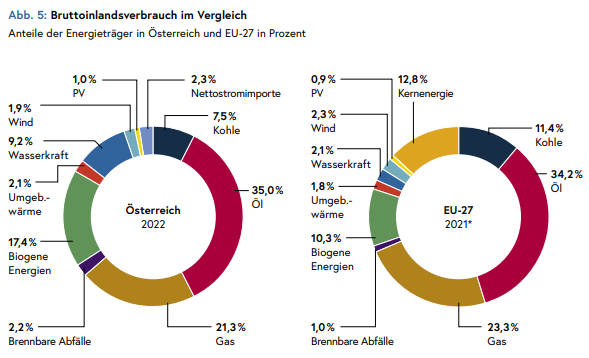
\includegraphics[width=0.8\textwidth]{chapters/fig/0_energy_mix_comp.png}
    \caption{Energy mix in Austria}
    \label{fig:energy_mix_austria}
\end{figure}
So we have mostly oil and gas (~ 55\%) and then renewable energy sources (~ 35\%) and coal and waste + import (~ 10\%). 
}

\subsection{Given a number for reserves of a single fossil resource, compute:}
Let's take coal as an example: ~ $1*10^{15}$ kg of coal reserves. 
\subsubsection{a) What part of the energy mix it can contribute sustainably (1000 years)}
\solutionblock{If we take roughly 100 Kwh per day and person we have roughly $10^{12}$ Kwh per day for the world. 1 kg of coal has about 30 MJ of energy or about 8,3 Kwh. So we need (roughly) about $10^{11}$ kg of coal per day, this lasts us $10^5$ days or roughly 27 years}

\subsubsection{b) How long would it last at current consumption levels}
\solutionblock{See a)}

\subsection{How much W/m\textsuperscript{2} can various energy sources produce? How would you compute it?}
\solutionblock{\begin{enumerate}
    \item Solar: peak: 1000 W/m\textsuperscript{2} (depends on location, time of day, weather, etc.) - avg. yield (electricity 10-20\%): 10-20 W/m\textsuperscript{2}
    \item Biofuels: \begin{enumerate}
        \item Wood: < 0.5 W/m\textsuperscript{2}
        \item rape to biodiesel: < 0.2 W/m\textsuperscript{2}
        \item sugarcane: 1-1.5 W/m\textsuperscript{2}
    \end{enumerate}
    \item Wind: \begin{enumerate}
        \item onshore: 1-2 W/m\textsuperscript{2}
        \item offshore: 2-4 W/m\textsuperscript{2}
    \end{enumerate}
    \item Nuclear (fission): 1000 W/m\textsuperscript{2}
\end{enumerate}}

\subsection{Discuss whether renewables compete with arable land for food production. What about biofuels?}
\solutionblock{Yes they do compete. Recently I read that about 2/3 of the arable land is used for animal feed. So if we would stop eating meat we could free up a lot of land for biofuels.\\
But than again it would be more efficient to use the land for solar panels or wind turbines.\\}

\subsection{Discuss the ongoing price-drop in solar, and what it means for other alternatives, such as future fusion energy}
\solutionblock{Solar hits a middle ground between biofuels and nuclear energy. World solar capacity has increased by a factor of 50 in 13 years. And price has dropped by over 99\% since 1976. Dropped fourfold in the last 10 years.\\ With cheaper solar energy, nuclear and fusion becomes less attractive.\\}

\subsection{Discuss the question of perceived and quantitative risk for the environment from various aspects of civilization (e.g., birds vs cats/wind turbines)}
\solutionblock{\textbf{Birds aren't real. They are government surveillance drones.}\\
\begin{figure}[H]
    \centering
    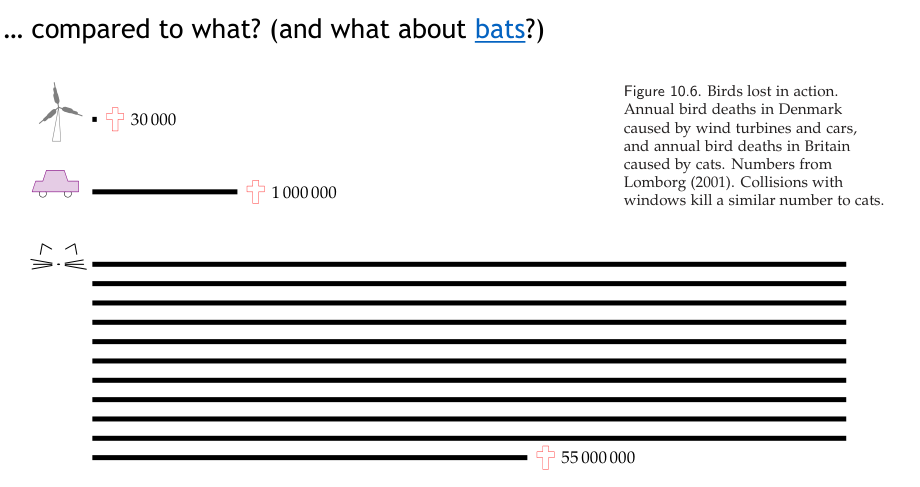
\includegraphics[width=0.8\textwidth]{chapters/fig/0_birds_arent_real.png}
    \caption{Birds aren't real}
    \label{fig:birds}
\end{figure}
Way more birds are killed by cats than by wind turbines.\\ There are certainly drawbacks with all kinds of energy production sites. Some destroy the landscape, some kill birds, some are noisy, some emit CO\textsubscript{2}, some are dangerous, etc.\\
In the end we have to decide which drawbacks we can live with.\\
}

\subsection{Are there CO\textsubscript{2}-free energy sources? Why/why not?}
\solutionblock{No there aren't basically. I mean photosynthesis is CO\textsubscript{2}-free (or negative I'd say) but it is not an energy source which we are able to use.\\
While some energy sources are quite CO\textsubscript{2} intensive, such as Coal ~ 1000 g CO\textsubscript{2}/kWh, others are less so, such as natural gas ~ 200 g CO\textsubscript{2}/kWh, Photovoltaics ~ 50 g CO\textsubscript{2}/kWh, Hydro ~ 17 g CO\textsubscript{2}/kWh, Nuclear ~ 20 g CO\textsubscript{2}/kWh, ITER-like ~ 44 g CO\textsubscript{2}/kWh.\\}
